% !TeX root = ../../金融经济学习题讲义.tex
% 源 PDF：references/金融经济学/史上最全最完整的金融经济学答案(王江版).pdf，页 44–53（印刷页 43–52）

\chapter{完全市场中的资源配置与资产价格}

\begin{problem}
\problemno{10.1*} 考虑一个两期（$t=0,\,1$）、两个状态（$\omega=a,\,b$），存在 $K$ 个参与者的经济。状态 $a$ 发生的概率为 $\pi_{a}$ 而状态 $b$ 发生的概率为 $\pi_{b}$。所有参与者都是不满足的且严格风险厌恶的。他们期望效用有如下形式：
\[
    u_{k}(c_{k,0})+\pi_{a}u_{k}(c_{k,a})+\pi_{b}u_{k}(c_{k,b}),\quad k=1,\dots,K.
\]
参与者 $k$ 的禀赋是 $\begin{bmatrix}e_{k,0} \\ e_{k,a} \\ e_{k,b}\end{bmatrix}$。整个经济的总禀赋是 $\begin{bmatrix}C_{0} \\ C_{a} \\ C_{b}\end{bmatrix}$，其中 $C_{s}=\sum_{k}e_{k,s}$，$s=0,a,b$。假设 $C_{a}>C_{b}$。假设市场上交易的 Arrow--Debreu 状态或有要求权的集合是完全的。令 $\phi_{a}$ 和 $\phi_{b}$ 分别是状态 $a$ 和状态 $b$ 的状态价格。
\begin{enumerate}[label=(\alph*)]
    \item 定义这个经济的均衡。简要讨论均衡的存在性和唯一性。
    \item 令代表性参与者的（间接）期望效用函数为
    \[
        u(C_{0})+\pi_{a}u(C_{a})+\pi_{b}u(C_{b})
    \]
    且 $u'''(\cdot)<0$。当以下变量变化而其它变量保持不变时，状态价格（$\phi_{a}$ 和 $\phi_{b}$）、它们的比例（$\phi_{a}/\phi_{b}$）和无风险利率如何变化（上升或下降）？给出证明。
    \begin{itemize}
        \item $C_{0}$ 上升；
        \item $C_{a}$ 上升；
        \item $C_{b}$ 上升；
        \item $C_{a}$ 和 $C_{b}$ 同比例上升；
        \item $C_{a}-C_{b}$ 上升（禀赋的风险上升）。
    \end{itemize}
\end{enumerate}
\end{problem}
\begin{solution}
\begin{enumerate}[label=(\alph*)]
    \item 这个经济的均衡是存在状态价格 $\begin{bmatrix}\phi_{a} \\ \phi_{b}\end{bmatrix}$，使得
    \begin{enumerate}[label=（\arabic*）]
        \item 给定状态价格和自己的禀赋，每个参与者都最优化地选择自己的消费；
        \item 市场出清：$\sum c_{k,0}=C_{0}$，$\sum c_{k,a}=C_{a}$，$\sum c_{k,b}=C_{b}$。由于市场是完全的，而参与者的效用函数是严格凹的，因而市场均衡是存在且唯一的。
    \end{enumerate}
    \item 我们知道
    \[
        \begin{aligned}
            \phi_{a}&=\pi_{a}u'(C_{a})/u'(C_{0}),\quad
            \phi_{b}=\pi_{b}u'(C_{b})/u'(C_{0}),\quad
            \frac{\phi_{a}}{\phi_{b}}=\frac{\pi_{a}u'(C_{a})}{\pi_{b}u'(C_{b})}\\
            r_{F}&=\frac{1}{\phi_{a}+\phi_{b}}-1=\frac{u'(C_{0})}{\pi_{a}u'(C_{a})+\pi_{b}u'(C_{b})}-1\\
            u'&>0,\quad u''<0,\quad u'''<0
        \end{aligned}
    \]
    \begin{itemize}
        \item 因为 $u''<0$，故 $C_{0}$ 上升使得 $u'(C_{0})$ 减小；$\phi_{a}$，$\phi_{b}$ 上升，$\phi_{a}/\phi_{b}$ 不变，$r_{F}$ 下降；
        \item 因为 $C_{a}$ 上升使得 $u'(C_{a})$ 下降，因而 $\phi_{a}$，$\phi_{a}/\phi_{b}$ 下降，$\phi_{b}$ 不变，$r_{F}$ 上升；
        \item 类似地，因为 $C_{b}$ 上升使得 $u'(C_{b})$ 下降，因而 $\phi_{b}$ 下降，$\phi_{a}/\phi_{b}$ 上升，$\phi_{a}$ 不变，$r_{F}$ 上升；
        \item $\phi_{a}$，$\phi_{b}$ 下降，$r_{F}$ 上升。现在考虑 $\phi_{a}/\phi_{b}$：
        \[
            \frac{\phi_{a}'/\phi_{b}'}{\phi_{a}/\phi_{b}}=\frac{u'(kC_{a})/u'(kC_{b})}{u'(C_{a})/u'(C_{b})}=\frac{u'(kC_{a})/u'(C_{a})}{u'(kC_{b})/u'(C_{b})}
        \]
        令 $f(x)=\dfrac{u'(kx)}{u'(x)}$，那么 $f'(x)=\dfrac{u'(kx)}{xu'(x)}(-R(kx)+R(x))$，其中 $R(x)$ 是相对风险厌恶系数，可以证明当 $u'''<0$ 时，$R(x)$ 是递增的，因而 $f'(x)<0$。因此，如果 $C_{a}>C_{b}$，那么 $\phi_{a}/\phi_{b}$ 会下降，反之则会上升。
        \item $\phi_{a}$，$\phi_{a}/\phi_{b}$ 下降，$\phi_{b}$ 上升，现在考虑 $r_{F}$。不妨假设 $C_{a}>C_{b}$，现在 $C_{a}$ 上升，$C_{b}$ 下降使得 $\phi_{a}C_{a}+\phi_{b}C_{b}=\tilde{C}$ 保持不变。考虑 $\phi_{a}u'(C_{a})+\phi_{b}u'(C_{b})=\phi_{a}u'(C_{a})+\phi_{b}u'(\tilde{C}-\pi_{a}C_{a})$，对 $C_{a}$ 求导可得 $\pi_{a}[u''(C_{a})-u''(C_{b})]$，因为 $u'''<0$，故 $r_{F}$ 上升。
    \end{itemize}
\end{enumerate}
\end{solution}

\begin{problem}
\problemno{10.2**} 考虑一个含有参与者 $k=1,\dots,K$ 的 Arrow--Debreu 经济。参与者 $k$ 具有形式为 $u_{k,0}(c_{0})+\mathrm{E}[u_{k,1}(c_{1})]$ 的效用函数，对于所有 $k$，$u_{0,k}$ 和 $u_{k,1}$ 是严格递增和严格凹的。$f_{k}^{0}$ 和 $f_{k}$ 是在给定权重集合 $\lambda=\{\lambda_{1},\dots,\lambda_{K}\}$ 下对于参与者 $k$ 的 Pareto 最优分配规则。定义 $u_{0}$ 和 $u_{1}$ 如下
\[
    u_{0}'(x)=\lambda_{k}u_{k,0}(f_{k}^{0}(x)),\qquad u_{1}'(x)=\lambda_{k}u_{k,1}(f_{k}(x)).
\]
\begin{enumerate}[label=(\alph*)]
    \item 证明 $u_{0}$ 和 $u_{1}$ 是严格递增和严格凹的。
    \item 证明 $u_{0}(c_{0})+\mathrm{E}[u_{1}(c_{1})]$ 是代表性参与者的效用函数。
    \item 证明如果所有参与者都是绝对风险厌恶递减的，那么以上定义的代表性参与者的效用函数也是绝对风险厌恶递减的。
\end{enumerate}
\end{problem}
\begin{solution}
\begin{enumerate}[label=(\alph*)]
    \item $u_{1}'(x)=\lambda_{k}u_{k,1}'(f_{k}(x))>0$，$u_{1}''(x)=\lambda_{k}u_{k,1}''(f_{k}(x))f_{k}'(x)<0$，这是因为 $u_{k}''<0$ 而 $f_{k}'>0$（定理 10.6），因而 $u_{1}$ 是严格递增且凹的，同样可以证明 $u_{0}$ 是严格递增且凹的；
    \item 由 (10.14) 式我们知道，代表性参与者的效用函数满足
    \[
        u_{0}'(x)=\lambda_{k}u_{k,0}(f_{k}^{0}(x)),\qquad u_{1}'(x)=\lambda_{k}u_{k,1}(f_{k}(x)),\quad\forall k
    \]
    因此（除相差一个常数为）$u_{0}(c_{0})+\mathrm{E}[u_{1}(c_{1})]$ 就是代表性参与者的效用函数。
    \item 由于 $u_{0}$、$u_{1}$ 的证明方法完全一样，因而我们忽略下标 $0$、$1$。如果参与者是绝对风险厌恶递减的，那么有 $[u_{k}'']^{2}-u_{k}'u_{k}'''<0$。对于代表性参与者有
    \[
        A(x)=-\frac{u_{k}''(f_{k}(x))f_{k}'(x)}{u_{k}'(f_{k}(x))}
    \]
    那么
    \[
        A'(x)=\frac{[u_{k}'']^{2}[f_{k}']^{2}-u_{k}'u_{k}''f_{k}''-u_{k}'u_{k}'''[f_{k}']^{2}}{[u_{k}']^{2}}
    \]
    因此，
    \[
        f_{k}''=\frac{A'(x)[u_{k}']^{2}+u_{k}'u_{k}'''[f_{k}']^{2}-[u_{k}'']^{2}[f_{k}']^{2}}{-u_{k}'u_{k}''}
    \]
    对于分配规则，我们有
    \[
        \sum f_{k}(x)=x,\quad \sum f_{k}'(x)=1,\quad \sum f_{k}''(x)=0
    \]
    因此我们有
    \[
        A'(x)=\sum\frac{[f_{k}']^{2}\bigl([u_{k}'']^{2}-u_{k}'u_{k}'''\bigr)}{-u_{k}'u_{k}''}\Big/\sum\frac{-u_{k}'}{u_{k}''}<0
    \]
    因而代表性参与者的效用函数也是绝对厌恶递减的。
\end{enumerate}
\end{solution}

\begin{problem}
\problemno{10.3*} 在 1 期，经济有两个可能状态 $a$ 和 $b$。它们的发生的概率分别为 $\pi$ 和 $1-\pi$。市场有两只交易证券，证券 1 和 2，支付如下：
\begin{center}
\begin{tabular}{@{}c@{\hspace{2.5em}}c@{}}
证券 1：
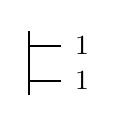
\begin{tikzpicture}[x=1.15em,y=1.15em,baseline=(current bounding box.center)]
    \draw[thick] (-0.15,-1) -- (-0.15,1);
    \draw[thick] (-0.15,0.55) -- (0.85,0.55);
    \draw[thick] (-0.15,-0.55) -- (0.85,-0.55);
    \node[anchor=west] at (1.0,0.55) {$1$};
    \node[anchor=west] at (1.0,-0.55) {$1$};
\end{tikzpicture}
&
证券 2：
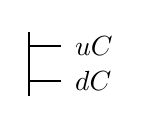
\begin{tikzpicture}[x=1.15em,y=1.15em,baseline=(current bounding box.center)]
    \draw[thick] (-0.15,-1) -- (-0.15,1);
    \draw[thick] (-0.15,0.55) -- (0.85,0.55);
    \draw[thick] (-0.15,-0.55) -- (0.85,-0.55);
    \node[anchor=west] at (1.0,0.55) {$uC$};
    \node[anchor=west] at (1.0,-0.55) {$dC$};
\end{tikzpicture}
\end{tabular}
\end{center}
其中 $C>0$ 且 $0<d<u$。因此，证券 1 是无风险债券而证券 2 是风险证券，我们可以称它为股票。经济中有参与者 $k=1,\dots,K$。参与者 $k$ 的禀赋是 $s_{k}C$ 单位的当期消费、0 单位的证券 1 和 $s_{k}$ 单位的证券 2，其中 $s_{k}>0$ 且 $\sum_{k}s_{k}=1$。所有参与者具有如下的期望效用函数：
\[
    U_{k}(c_{k})=\log c_{k,0}+\rho\bigl[\pi\log c_{k,1a}+(1-\pi)\log c_{k,1b}\bigr]
\]
其中 $\rho>0$。
\begin{enumerate}[label=(\alph*)]
    \item 证明证券市场是完全的。
    \item 求解每一参与者的最优消费/投资选择。
    \item 求解均衡证券价格。
    \item 将价格过程与期权定价中的二叉树模型相比较，你能得到什么结论？
\end{enumerate}
\end{problem}
\begin{solution}
\begin{enumerate}[label=(\alph*)]
    \item 市场上有两只支付独立的证券，而状态数目恰为 2，因而市场是完全的。
    \item 参与者 $k$ 面临的问题是
    \[
        \begin{aligned}
            &\max_{\{c_{k,0},c_{k,1a},c_{k,1b}\}}\ \log c_{k,0}+\rho\bigl[\pi\log c_{k,1a}+(1-\pi)\log c_{k,1b}\bigr]\\
            &\quad\text{s.t.}\quad c_{k,0}+\phi_{a}c_{k,1a}+\phi_{b}c_{k,1b}=S_{k}C(1+\phi_{a}u+\phi_{b}d)
        \end{aligned}
    \]
    可以求得
    \[
        \begin{aligned}
            c_{k,0}&=\frac{S_{k}C(1+\phi_{a}u+\phi_{b}d)}{1+\rho}\\
            c_{k,1a}&=\frac{\rho\pi S_{k}C(1+\phi_{a}u+\phi_{b}d)}{\phi_{a}(1+\rho)}\\
            c_{k,1b}&=\frac{\rho(1-\pi)S_{k}C(1+\phi_{a}u+\phi_{b}d)}{\phi_{b}(1+\rho)}
        \end{aligned}
    \]
    当市场达到均衡时：
    \[
        \begin{aligned}
            \sum c_{k,0}&=\sum S_{k}C=C\\
            \sum c_{k,1a}&=\sum S_{k}uC=uC\\
            \sum c_{k,1b}&=\sum S_{k}dC=dC
        \end{aligned}
    \]
    因此求得
    \[
        \begin{aligned}
            \phi_{a}&=\frac{\rho\pi}{u},\qquad\phi_{b}=\frac{\rho(1-\pi)}{d}\\
            c_{k,0}&=S_{k}C,\qquad c_{k,1a}=S_{k}uC,\qquad c_{k,1b}=S_{k}dC
        \end{aligned}
    \]
    \item 债券价格为 $\dfrac{\rho\pi}{u}+\dfrac{\rho(1-\pi)}{d}$，股票价格为 $\rho C$。
    \item 在二叉树模型中，债券、股票的价格都是给定的，因而状态价格只由债券、股票的支付给定，得到的是部分均衡的结果；在这个模型中，价格是通过市场均衡求得的，因而状态价格还与参与者的效用函数、时间偏好系数、状态发生的概率有关，得到的是一般均衡的结果。
\end{enumerate}
\end{solution}

\begin{problem}
\problemno{10.4**} 继续考虑练习 10.3 定义的经济，
\begin{enumerate}[label=(\alph*)]
    \item 构建代表性参与者。
    \item 计算在代表性参与者（即中央计划者）的效用函数中每个参与者的权重。它依赖于什么？为什么？
    \item 证明代表性参与者的偏好与禀赋在参与者之间的分布无关。
    \item 用基于消费的 CAPM 为两只证券定价。
    \item 计算无风险收益和股票的风险溢价。
    \item 利率和股票的风险溢价依赖于什么？解释它们对经济原生变量：当前消费水平、消费增长率的期望值 $\mathrm{E}[\tilde{C}_{1}/C_{0}]$、消费增长率的波动率 $\mathrm{Var}[\tilde{C}_{1}/C_{0}]$ 以及时间折现系数 $\rho$ 的依赖性？
\end{enumerate}
\end{problem}
\begin{solution}
\begin{enumerate}[label=(\alph*)]
    \item 由第二题我们知道，代表性参与者的效用函数满足
    \[
        u_{0}'(C)=\mu_{k}u_{k,0}'(c_{k})=\frac{\mu_{k}}{c_{k}}=\frac{\mu_{k}}{S_{k}C},\quad\forall k
    \]
    因此 $\mu_{k}=S_{k}$，$u_{0}'(C)=\dfrac{1}{C}$，$u_{0}(C)=\log C$，同样地，$u_{1}(C)=\log C$；因而代表性参与者的效用函数为
    \[
        \log C_{0}+\rho\bigl[\pi\log C_{1a}+(1-\pi)\log C_{1b}\bigr]
    \]
    \item 参与者 $k$ 的权重是 $S_{k}$，即他的禀赋占总禀赋的比例。如果参与者拥有的资源愈多，在均衡条件下，他的消费越多，权重也越大；
    \item 代表性参与者的偏好与 $S_{k}$ 无关，即与禀赋在参与者之间的分布无关；
    \item 由 (10.16) 式我们有：
    \[
        \begin{aligned}
            \text{债券价格为：}&\quad
            \pi\frac{\rho C}{uC}+(1-\pi)\frac{\rho C}{dC}=\rho\Bigl[\frac{\pi}{u}+\frac{1-\pi}{d}\Bigr]\\
            \text{股票价格为：}&\quad
            \pi\frac{\rho C}{uC}uC+(1-\pi)\frac{\rho C}{dC}dC=\rho C
        \end{aligned}
    \]
    \item 无风险收益率为
    \[
        r_{F}=1\big/\Bigl(\rho\Bigl[\frac{\pi}{u}+\frac{1-\pi}{d}\Bigr]\Bigr)-1
    \]
    风险溢价为
    \[
        p=\Bigl(\frac{\pi}{u}+\frac{1-\pi}{d}\Bigr)\big/\rho-1\big/\Bigl(\rho\Bigl[\frac{\pi}{u}+\frac{1-\pi}{d}\Bigr]\Bigr)
    \]
    \item 如果 $u$，$d$ 与 1 的距离很小，我们可以把风险溢价写成 $p=\dfrac{\mathrm{E}[\tilde{C}_{1}]/C_{0}}{\rho}-r_{F}$，其中 $r_{F}=1\big/\bigl\{\rho\bigl[\mathrm{Var}[\tilde{C}_{1}/C_{0}]-2\mathrm{E}[\tilde{C}_{1}/C_{0}]+3\bigr]\bigr\}$。无风险利率依赖于时间偏好系数 $\rho$、消费增长率的波动率 $\mathrm{Var}[\tilde{C}_{1}/C_{0}]$、以及消费增长率的期望值 $\mathrm{E}[\tilde{C}_{1}/C_{0}]$。当 $\rho$ 减小时，参与者偏好于当前消费，而为了吸引投资者储蓄以平衡当前消费和未来消费，利率 $r_{F}$ 应该上升；当未来消费的风险上升时，为规避未来消费的风险，参与者对债券的需求上升，其价格上升、利率下降；当 $\mathrm{E}[\tilde{C}_{1}/C_{0}]$ 上升时，人们倾向于在时间上平滑消费水平，即增加当前消费，为吸引投资，利率上升。至于风险溢价，当 $\rho$ 上升时，参与者倾向于未来消费，因而债券、股票的需求量都会上升，利率和股票收益率都减小，而且对两者的影响相对一样，因而风险溢价变小（风险溢价一般都是正的）。当 $\mathrm{E}[\tilde{C}_{1}/C_{0}]$ 变大时，参与者倾向于当前消费，因而对债券和股票的需求量都减小，两者的价格都下降、收益率都上升，对风险溢价的影响是不确定的，但当 $\mathrm{E}[\tilde{C}_{1}/C_{0}]$ 较小时，利率上升更快，风险溢价会变小。当 $\mathrm{Var}[\tilde{C}_{1}/C_{0}]$ 变大时，因为股票的风险和禀赋的风险完全一致，为了减少未来消费的波动，人们对债券的需求增加而对股票的需求减少，因而债券收益率下降而股票收益上升，风险溢价上升。
\end{enumerate}
\end{solution}

\begin{problem}
\problemno{10.5} 继续前面练习中的经济。
\begin{enumerate}[label=(\alph*)]
    \item 求解以证券 2 为标的资产、执行价格为 $K$ 的看涨期权的价格。
    \item 证明基于消费的 CAPM 也适用于期权。
\end{enumerate}
\end{problem}
\begin{solution}
\begin{enumerate}[label=(\alph*)]
    \item 不失一般性，假设 $dC\le K\le uC$，期权的支付为 $\begin{bmatrix}uC-K \\ 0\end{bmatrix}$，用复制的方法可以求得期权的价格为 $\dfrac{\rho\pi}{u}(uC-K)$；
    \item 而用 CCAPM 定价，期权的价格为
    \[
        \pi\frac{\rho C}{uC}[uC-K]_{+}+(1-\pi)\frac{\rho C}{dC}[dC-K]_{+}=\frac{\rho\pi}{u}(uC-K)
    \]
    因而 CCAPM 成立。
\end{enumerate}
\end{solution}

\begin{problem}
\problemno{10.6**} 在 1 期，经济有两个可能状态 $a$ 和 $b$。它们的发生概率分别为 $\pi$ 和 $1-\pi$。市场有两只交易证券，证券 1 和 2，支付如下：
\begin{center}
\begin{tabular}{@{}c@{\hspace{2.5em}}c@{}}
证券 1：
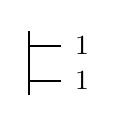
\begin{tikzpicture}[x=1.15em,y=1.15em,baseline=(current bounding box.center)]
    \draw[thick] (-0.15,-1) -- (-0.15,1);
    \draw[thick] (-0.15,0.55) -- (0.85,0.55);
    \draw[thick] (-0.15,-0.55) -- (0.85,-0.55);
    \node[anchor=west] at (1.0,0.55) {$1$};
    \node[anchor=west] at (1.0,-0.55) {$1$};
\end{tikzpicture}
&
证券 2：
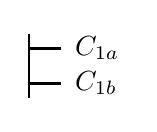
\begin{tikzpicture}[x=1.15em,y=1.15em,baseline=(current bounding box.center)]
    \draw[thick] (-0.15,-1) -- (-0.15,1);
    \draw[thick] (-0.15,0.55) -- (0.85,0.55);
    \draw[thick] (-0.15,-0.55) -- (0.85,-0.55);
    \node[anchor=west] at (1.0,0.55) {$C_{1a}$};
    \node[anchor=west] at (1.0,-0.55) {$C_{1b}$};
\end{tikzpicture}
\end{tabular}
\end{center}
其中 $C>0$ 且 $0<d<u$。因此，证券 1 是无风险债券而证券 2 是风险证券，我们可以称它为股票。经济中有参与者 $k=1,\dots,K$。参与者 $k$ 的禀赋是 $s_{k}C_{0}$ 单位的当期消费、0 单位的证券 1 和 $s_{k}$ 单位的证券 2，其中 $s_{k}>0$ 且 $\sum_{k}s_{k}=1$。所有参与者具有如下的期望效用函数：
\[
    U_{k}(c_{k})=-e^{-\alpha c_{k,0}}-\rho\bigl[\pi e^{-\alpha c_{k,1a}}+(1-\pi)e^{-\alpha c_{k,1b}}\bigr]
\]
其中 $\rho>0$。
\begin{enumerate}[label=(\alph*)]
    \item 证明证券市场是完全的。
    \item 求解每一参与者的最优消费/投资选择。
    \item 求解均衡证券价格。
\end{enumerate}
\end{problem}
\begin{solution}
\begin{enumerate}[label=(\alph*)]
    \item 有 2 个可能状态，而支付独立的状态数目恰为 2，因此证券市场是完全的；
    \item 假设状态价格为 $\begin{bmatrix}\phi_{a} \\ \phi_{b}\end{bmatrix}$；考虑参与者 $k$，他的优化问题是
    \[
        \begin{aligned}
            &\max_{c_{k,0},\,c_{k,1a},\,c_{k,1b}}\ -e^{-\alpha c_{k,0}}-\rho\bigl[\pi e^{-\alpha c_{k,1a}}+(1-\pi)e^{-\alpha c_{k,1b}}\bigr]\\
            &\quad\text{s.t.}\quad c_{k,0}+\phi_{a}c_{k,1a}+\phi_{b}c_{k,1b}=s_{k}C_{0}+\phi_{a}s_{k}C_{1a}+\phi_{b}s_{k}C_{1b}
        \end{aligned}
    \]
    令 $W=C_{0}+\phi_{a}C_{1a}+\phi_{b}C_{1b}$ 为经济中的总财富。求解优化问题可得参与者的消费选择为
    \[
        \begin{aligned}
            c_{k,0}&=\frac{1}{\alpha}\log\alpha-\frac{\beta-\alpha s_{k}W}{\alpha(1+\phi_{a}+\phi_{b})}\\
            c_{k,1a}&=\frac{1}{\alpha}\log\frac{\rho\pi\alpha}{\phi_{a}}-\frac{\beta-\alpha s_{k}W}{\alpha(1+\phi_{a}+\phi_{b})}\\
            c_{k,1b}&=\frac{1}{\alpha}\log\frac{\rho(1-\pi)\alpha}{\phi_{b}}-\frac{\beta-\alpha s_{k}W}{\alpha(1+\phi_{a}+\phi_{b})}
        \end{aligned}
    \]
    其中，$\beta=\log\alpha+\phi_{a}\log\dfrac{\rho\pi\alpha}{\phi_{a}}+\phi_{b}\log\dfrac{\rho(1-\pi)\alpha}{\phi_{b}}$；
    \item 市场出清条件是
    \[
        \begin{aligned}
            \sum c_{k,0}&=C_{0}\\
            \sum c_{k,1a}&=C_{1a}\\
            \sum c_{k,1b}&=C_{1b}
        \end{aligned}
    \]
    由此可以求得均衡状态价格为
    \[
        \begin{aligned}
            \phi_{a}&=\rho\pi e^{-\frac{\alpha}{K}(C_{1a}-C_{0})}\\
            \phi_{b}&=\rho(1-\pi)e^{-\frac{\alpha}{K}(C_{1b}-C_{0})}
        \end{aligned}
    \]
    因而债券的均衡价格为 $\phi_{a}+\phi_{b}$，股票的均衡价格为 $\phi_{a}C_{1a}+\phi_{b}C_{1b}$；在均衡条件下，参与者 $k$ 的最优消费选择为
    \[
        \begin{aligned}
            c_{k,0}^{*}&=\frac{1}{K}C_{0}+\Bigl(s_{k}-\frac{1}{K}\Bigr)\frac{W}{1+\phi_{a}+\phi_{b}}\\
            c_{k,1a}^{*}&=\frac{1}{K}C_{1a}+\Bigl(s_{k}-\frac{1}{K}\Bigr)\frac{W}{1+\phi_{a}+\phi_{b}}\\
            c_{k,1b}^{*}&=\frac{1}{K}C_{1b}+\Bigl(s_{k}-\frac{1}{K}\Bigr)\frac{W}{1+\phi_{a}+\phi_{b}}
        \end{aligned}
    \]
    在 0 期他持有的无风险债券、股票的头寸分别为
    \[
        \begin{aligned}
            \theta_{B}&=\Bigl(s_{k}-\frac{1}{K}\Bigr)\frac{W}{1+\phi_{a}+\phi_{b}}\\
            \theta_{S}&=\frac{1}{K}-s_{k}.
        \end{aligned}
    \]
\end{enumerate}
\end{solution}

\begin{problem}
\problemno{10.7**} 继续考虑练习 10.6 定义的经济
\begin{enumerate}[label=(\alph*)]
    \item 构建代表性参与者。
    \item 计算在代表性参与者（即中央计划者）的效用函数中每个参与者的权重。它依赖于什么？为什么？
    \item 证明代表性参与者的偏好与禀赋在参与者之间的分布无关。
    \item 用基于消费的 CAPM 为两只证券定价。
    \item 计算无风险收益和股票的风险溢价，现在风险溢价的定义为 $\mathrm{E}[\tilde{S}_{1}]-(1+r_{F})S_{0}$。即一股股票的绝对超额收益。
    \item 利率和股票的风险溢价依赖于什么？解释它们对经济原生变量：当前消费水平、消费增长的期望值 $\mathrm{E}[\tilde{C}_{1}/C_{0}]$、消费增长的波动率 $\mathrm{Var}[\tilde{C}_{1}/C_{0}]$ 以及时间折现系数 $\rho$ 的依赖性？
    \item 求解以证券 2 为标的资产、执行价格为 $K$ 的看涨期权的价格。
\end{enumerate}
\end{problem}
\begin{solution}
\begin{enumerate}[label=(\alph*)]
    \item 因为每个参与者的 0、1 期效用函数只差时间偏好系数 $\rho$，因而代表性参与者的 0、1 期效用函数只差时间偏好系数 $\rho$；假设中央计划者问题中参与者 $k$ 的权重为 $\mu_{k}>0$，代表性参与者的 0 期效用函数为 $u(C_{0})$，那么
    \[
        \begin{aligned}
            u'(C_{0})
            &=\mu_{k}u_{k}'(c_{k,0})\\
            &=\mu_{k}\alpha e^{-\alpha\bigl(\frac{1}{K}C_{0}+\bigl(s_{k}-\frac{1}{K}\bigr)\frac{W}{1+\phi_{a}+\phi_{b}}\bigr)}\\
            &=e^{-\alpha\frac{C_{0}}{K}}\Bigl(\alpha\mu_{k}e^{-\alpha\bigl(s_{k}-\frac{1}{K}\bigr)\frac{W}{1+\phi_{a}+\phi_{b}}}\Bigr),\quad\forall k
        \end{aligned}
    \]
    因此，$\alpha\mu_{k}e^{-\alpha\bigl(s_{k}-\frac{1}{K}\bigr)\frac{W}{1+\phi_{a}+\phi_{b}}}$ 是与 $k$ 无关的常数，即 $\mu_{k}$ 与 $e^{\frac{\alpha}{1+\phi_{a}+\phi_{b}}s_{k}}$ 成正比，而且代表性参与者的效用函数具有负指数形式 $u(C_{0})=-e^{-\alpha\frac{C_{0}}{K}}$，因此，代表性参与者的效用函数为
    \[
        -e^{-\alpha\frac{C_{0}}{K}}-\rho\Bigl[\pi e^{-\alpha\frac{C_{1a}}{K}}+(1-\pi)e^{-\alpha\frac{C_{1b}}{K}}\Bigr]
    \]
    \item 权重 $\mu_{k}$ 与 $e^{\frac{\alpha}{1+\phi_{a}+\phi_{b}}s_{k}}$ 成正比，依赖于参与者的禀赋参数 $s_{k}$，即他的禀赋占总禀赋的比例。如果参与者拥有的资源愈多，在均衡条件下，他的消费越多，权重也越大；
    \item 代表性参与者的偏好与 $s_{k}$ 无关，即与禀赋在参与者之间的分布无关；
    \item
    \[
        \begin{aligned}
            \text{债券价格为：}&\quad
            \rho\pi\frac{\alpha e^{-\alpha\frac{C_{1a}}{K}}}{\alpha e^{-\alpha\frac{C_{0}}{K}}}+\rho(1-\pi)\frac{\alpha e^{-\alpha\frac{C_{1b}}{K}}}{\alpha e^{-\alpha\frac{C_{0}}{K}}}\\
            &\qquad=\rho\Bigl[\pi e^{-\alpha\frac{C_{1a}-C_{0}}{K}}+(1-\pi)e^{-\alpha\frac{C_{1b}-C_{0}}{K}}\Bigr]\\
            \text{股票价格为：}&\quad
            \rho\pi\frac{\alpha e^{-\alpha\frac{C_{1a}}{K}}}{\alpha e^{-\alpha\frac{C_{0}}{K}}}C_{1a}+\rho(1-\pi)\frac{\alpha e^{-\alpha\frac{C_{1b}}{K}}}{\alpha e^{-\alpha\frac{C_{0}}{K}}}C_{1b}\\
            &\qquad=\rho\Bigl[\pi e^{-\alpha\frac{C_{1a}-C_{0}}{K}}C_{1a}+(1-\pi)e^{-\alpha\frac{C_{1b}-C_{0}}{K}}C_{1b}\Bigr]
        \end{aligned}
    \]
    \item 无风险收益率为
    \[
        r_{F}=\frac{1}{\phi_{a}+\phi_{b}}-1=\frac{1}{\rho\Bigl[\pi e^{-\alpha\frac{C_{1a}-C_{0}}{K}}+(1-\pi)e^{-\alpha\frac{C_{1b}-C_{0}}{K}}\Bigr]}-1
    \]
    风险溢价为
    \[
        \begin{aligned}
            p&=\mathrm{E}[\tilde{S}_{1}]-(1+r_{F})S_{0}\\
            &=\pi C_{1a}+(1-\pi)C_{1b}-\frac{\phi_{a}C_{1a}+\phi_{b}C_{1b}}{\phi_{a}+\phi_{b}}\\
            &=\Bigl(\pi-\frac{\phi_{a}}{\phi_{a}+\phi_{b}}\Bigr)(C_{1a}-C_{1b})\\
            &=\frac{\pi(1-\pi)\bigl(e^{\alpha\frac{C_{1a}-C_{1b}}{K}}-1\bigr)}{\pi+(1-\pi)e^{\alpha\frac{C_{1a}-C_{1b}}{K}}}(C_{1a}-C_{1b})
        \end{aligned}
    \]
    \item 如果 $\tilde{g}=\tilde{C}_{1}/C_{0}-1$ 很小，而人均消费 $C_{0}/K$ 是很大，那么无风险利率可以写成
    \[
        r_{F}\doteq\frac{1}{\rho\Bigl[1-\alpha\frac{C_{0}}{K}\mathrm{E}[\tilde{g}]+\alpha^{2}\frac{C_{0}^{2}}{K^{2}}\bigl(\mathrm{Var}[\tilde{g}]+\mathrm{E}^{2}[\tilde{g}]\bigr)\Bigr]}
    \]
    可以看出，无风险利率依赖于时间偏好系数 $\rho$、消费增长率的波动率 $\mathrm{Var}[\tilde{C}_{1}/C_{0}]$、以及消费增长率的期望值 $\mathrm{E}[\tilde{C}_{1}/C_{0}]$。当 $\rho$ 减小时，参与者偏好于当前消费，而为了吸引投资者储蓄以平衡当前消费和未来消费，利率 $r_{F}$ 应该上升；当未来消费的风险上升时，为规避未来消费的风险，参与者对债券的需求上升，其价格上升、利率下降；当 $\mathrm{E}[\tilde{C}_{1}/C_{0}]$ 上升时，人们倾向于在时间上平滑消费水平，即增加当前消费，为吸引投资，利率上升。至于风险溢价，它只与 $C_{1a}-C_{1b}$ 有关，且是 $C_{1a}-C_{1b}$ 的增函数；某种意义上我们可以把 $C_{1a}-C_{1b}$ 作为未来禀赋风险的一种度量，也就是说，当未来禀赋的风险增加时，风险溢价增加，这是因为股票的风险和禀赋的风险完全一致，为了减少未来消费的波动，人们对债券的需求增加而对股票的需求减少，因而债券收益率下降而股票收益上升，风险溢价上升。
    \item 可以用 CCAPM 为期权定价
    \[
        \begin{aligned}
            c&=\rho\pi\frac{\alpha e^{-\alpha\frac{C_{1a}}{K}}}{\alpha e^{-\alpha\frac{C_{0}}{K}}}[C_{1a}-K]_{+}+\rho(1-\pi)\frac{\alpha e^{-\alpha\frac{C_{1b}}{K}}}{\alpha e^{-\alpha\frac{C_{0}}{K}}}[C_{1b}-K]_{+}\\
            &=\rho\Bigl[\pi e^{-\alpha\frac{C_{1a}-C_{0}}{K}}[C_{1a}-K]_{+}+(1-\pi)e^{-\alpha\frac{C_{1b}-C_{0}}{K}}[C_{1b}-K]_{+}\Bigr]
        \end{aligned}
    \]
\end{enumerate}
\end{solution}
